\documentclass[twoside,twocolumn]{article}
\usepackage{amsmath}
\usepackage{amsfonts}
\usepackage{amssymb}
\usepackage{graphicx}
\usepackage{blindtext} % Package to generate dummy text throughout this template 

\usepackage[hmarginratio=1:1,top=32mm,columnsep=20pt]{geometry} % Document margins
\usepackage[hang, small,labelfont=bf,up,textfont=it,up]{caption} % Custom captions under/above floats in tables or figures
\usepackage{booktabs} % Horizontal rules in tables
\usepackage{lettrine} % The lettrine is the first enlarged letter at the beginning of the text

\usepackage{enumitem} % Customized lists
\setlist[itemize]{noitemsep} % Make itemize lists more compact

\usepackage{abstract} % Allows abstract customization
\renewcommand{\abstractnamefont}{\normalfont\bfseries} % Set the "Abstract" text to bold
\renewcommand{\abstracttextfont}{\normalfont\small\itshape} % Set the abstract itself to small italic text

\usepackage{titlesec} % Allows customization of titles
\renewcommand\thesection{\Roman{section}} % Roman numerals for the sections
\renewcommand\thesubsection{\roman{subsection}} % roman numerals for subsections
\titleformat{\section}[block]{\large\scshape\centering}{\thesection.}{1em}{} % Change the look of the section titles
\titleformat{\subsection}[block]{\large}{\thesubsection.}{1em}{} % Change the look of the section titles

\usepackage{fancyhdr} % Headers and footers
\pagestyle{fancy} % All pages have headers and footers
\fancyhead{} % Blank out the default header
\fancyfoot{} % Blank out the default footer
\fancyhead[C]{Datos no estructurados $\bullet$ Enero 2021 $\bullet$ } % Custom header text
\fancyfoot[RO,LE]{\thepage} % Custom footer text

\usepackage{titling} % Customizing the title section

\usepackage{hyperref} % For hyperlinks in the PDF

%----------------------------------------------------------------------------------------
%	TITLE SECTION
%----------------------------------------------------------------------------------------

\setlength{\droptitle}{-4\baselineskip} % Move the title up

\pretitle{\begin{center}\Huge\bfseries} % Article title formatting
\posttitle{\end{center}} % Article title closing formatting
\title{DATOS NO ESTRUCTURADOS : Formas de extracción de datos no estructurados} % Article title
\author{MamaniPerez,LaTorre,CarpioTejada,YanquiChambilla,MamaniLaura}
\date{\today} % Leave empty to omit a date

\renewcommand{\maketitlehookd}
{%
\begin{abstract}
\noindent In the modern world of Big Data, unstructured data is the most abundant. They are so prolific because unstructured data can be of any kind: multimedia, images, audio, sensor data, text data, and much more. Unstructured simply means that these are data sets (typical large collections of files) that are not stored in a structured database format. Unstructured data has internal structure, but it is not predefined by data models. They can generate human beings or a machine, in textual or non-textual format.

\end{abstract}
}
%----------------------------------------------------------------------------------------

\begin{document}

% Print the title
\maketitle

%----------------------------------------------------------------------------------------
%	ARTICLE CONTENTS
%----------------------------------------------------------------------------------------

\section{Resumen}

\lettrine[nindent=0em,lines=2]{E}n el mundo moderno de Big Data, los datos no estructurados son los que más abundan. Son tan prolíficos porque los datos no estructurados pueden ser de cualquier índole: multimedia, imágenes, audio, datos de sensor, datos de texto y mucho más. No estructurado significa simplemente que se trata de conjuntos de datos (colecciones grandes típicas de archivos) que no se almacenan en un formato de base de datos estructurado. Los datos no estructurados tienen estructura interna, pero no están predefinidos por modelos de datos. Pueden generarlos los seres humanos o una máquina, en formato textual o no textual.


%------------------------------------------------
\section{Introducción}

 En el Presente artículo se analizará y mostrará sobre las formas de extracción de los datos no estructurados. Los datos no estructurados pueden definirse como datos, en cualquier forma, que no tengan un modelo o formato predefinido. Este tipo de datos se genera a partir de varias fuentes, incluidos audio, video, imágenes y texto.
La mayoría de las organizaciones cuentan con estrategias sólidas para administrar y analizar sus datos estructurados, pero el valor real radica en administrar esta nueva ola de contenido no estructurado. En esta publicación de blog, presentamos los fundamentos de las soluciones de administración de datos no estructurados para equipos de TI y propietarios de negocios.


%------------------------------------------------

\section{Desarrollo}

\subsection{¿Qué retos presenta el trabajo con datos no estructurados?}
La forma de pensar en cómo hacer frente a los retos de los datos no estructurados es preguntarse: ¿cómo hacen frente las empresas con enfoques tradicionales para gestionar los datos no estructurados? 
 
\subsection{Escalado}
Es común en muchas empresas encontrar conjuntos de datos no estructurados a la escala de decenas o cientos de miles de millones de elementos. Estos elementos, objetos o archivos pueden tener un tamaño de unos pocos bytes (por ejemplo, una lectura de temperatura desde un instrumento de línea de producción) a terabytes (por ejemplo, una imagen de movimiento de resolución de 8 K de longitud completa). La gestión de esta escala con los enfoques de archivos tradicionales pasa rápidamente de difícil a imposible, ya que se requieren más y más recursos para mantener un "equilibrio" de servidores, sistemas de archivos, cabinas, etc.


\subsection{Colaboración}
Cada vez más, estos conjuntos de datos masivos no estructurados proporcionan valor a medida que se comparten (por ejemplo, investigadores de varios hospitales que comparten un banco masivo común de secuencias genómicas). Con los enfoques tradicionales, la capacidad de compartir conjuntos masivos de datos no estructurados entre geografías, entidades corporativas, etc., ha requerido una replicación y una gobernanza extremadamente caras.

\subsection{¿Por qué es importante la extracción de datos y por qué necesita herramientas de extracción de datos?}
Muchas empresas están aprovechando las herramientas ETL para la gestión de datos y para la conversión de datos no estructurados a estructurados. Estas herramientas de consolidación de datos permiten a los usuarios de información romper los silos de datos, combinar datos de múltiples fuentes, convertirlos a un formato consistente y cargarlos en un destino de destino. Aunque los humanos pueden leer los datos no estructurados, las máquinas necesitan datos estructurados para procesarlos digitalmente. Por lo tanto, se requiere que los datos ETL no estructurados se extraigan de su fuente y se conviertan a un formato estructurado utilizando una solución automatizada de extracción de datos. El primer paso en el proceso ETL implica la extracción de datos, que básicamente ayuda a extraer datos estructurados de los no estructurados. Las herramientas y técnicas de extracción de datos adecuadas permiten que la información atrapada dentro de sistemas dispares se pueda estandarizar y preparar para futuras transformaciones, y los equipos de ETL pueden extraer información fácilmente de los datos.

\subsection{Formas de extracción de Datos}

•	Import.io 
\newline
Import.io es una aplicación web para convertir una página web en una API. Dada la simplicidad de la herramienta, su uso es muy intuitivo: simplemente introduciendo un enlace, automáticamente obtenemos toda la información de la web organizada en columnas (para lo que es necesario modelar las columnas y filtrar los contenidos no deseados o redundantes). Además, detecta paginación en los sitios web y permite descargar un fichero con los datos, integrarlos con otros servicios como Hojas de Cálculo de Google o Plot.ly o bien crear una API.
\newline
\newline
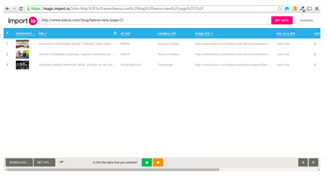
\includegraphics[width=7cm, height=5cm]{Image/bdimage.png}
\newline
\newline
\begin{itemize}
\item Scrapy
\newline
Scrapy es la herramienta de scraping más conocida. Es un framework complejo, no tan solo una librería. Guarda cierta similitud con Django, por ejemplo definiendo modelos de los datos, plugins, settings o la interacción mediante la línea de comandos para construir proyectos y ejecutarlos. Es un sistema muy flexible y abierto al desarrollo de extensiones adicionales.
\newline
Esta orientado a obtener información proveniente de páginas web y también realiza tareas de crawling. Es posible definir reglas para seguir enlaces o construir un sitemap. Las peticiones las realiza de forma asíncrona, por lo que es muy rápido y eficaz para paralelizar tareas. Tiene un gran número de utilidades para la exportación de los datos, llamados “Pipelines”. Es posible utilizar JSON, XML, CSV, objetos de Django, MongoDB o cualquier otro formato de almacenamiento disponible para Python. Scrapy es el más adecuado para trabajar con grandes cantidades de datos.
\newline
De manera adicional, podemos realizar scraping visual de páginas web, sin tener conocimientos de programación, con el plugin Portia.
\newline
\item 	Kimono Labs
\newline
Kimono Labs es otra aplicación para extracción visual de información. La aplicación es una extensión del navegador, un plugin. Una vez presente en una página web, abriendo Kimono, pasamos a un modo de selección. Es un proceso muy simple en el cual tenemos que elegir los datos deseados simplemente haciendo clic en un campo y confirmando la repetición del patrón.
\newline
También es compatible con sitios web que incluyen navegación paginada o carga dinámica basada en el movimiento de scroll. Una vez más, el resultado es una API accesible desde otros dispositivos.  
\newline

\includegraphics[width=7cm, height=5cm]{Image/bdimages.png}
\newline
\newline
Kimono Labs e Import.io son tecnologías muy similares, son competidores directos, pero su enfoque es muy distinto. Kimono es mucho más robusto y abierto para modelar los datos y obtener resultados más complejos y flexibles. Import.io en cambio es mucho más simple y efectivo en la mayoría de los casos de uso, pues no permite personalización. 
\newline
\newline
\item Tabula 
\newline
Tabula es una aplicación de escritorio para equipos Windows, Mac OSX y Linux, que proporciona a los desarrolladores e investigadores un método sencillo de extracción de datos desde un PDF a un archivo en formato CSV o Microsoft Excel para su modificación y visualización. Tabula es una herramienta muy utilizada en el periodismo de datos. 
\newline
\newline
Los pasos a seguir para utilizar Tabula:
\begin{itemize}
\item Cargar un PDF con la tabla de datos que se quiere exportar. 
\newline
\newline
\item Seleccionar la tabla con toda la información.
\newline
\newline
\item Seleccionar la opción de ‘Vista previa y extracción de datos’. Tabula escrapea los datos de la tabla y ofrece al usuario una vista previa de la información extraída para su comprobación.
\newline
\newline
\item  Pulsar el botón de ‘Exportar’.
\newline
\newline
\item Los datos se exportan a un archivo Microsoft Excel o bien un archivo LibreOffice si no disponemos de Microsoft Office.
\newline
\newline
\item  Tabula es un proyecto de código abierto disponible en GitHub.
\newline
\newline
\end{itemize}


\clearpage


\clearpage



\section{Conclusiones}
A nivel técnico, la comunidad tiende a desarrollar herramientas cada vez más especializadas. Hay pocos proyectos grandes que cuenten con soporte activo de la comunidad. Scrapy es un ejemplo de ello. Es una herramienta generalista, pero con un alto grado de eficiencia, facilidad para extenderlo y compatible con otras herramientas, lo que la convierte en una navaja suiza: útil en la mayoría de los contextos.

\section{Recomendaciones}

\item 1.- La principal recomendación para hacer scraping es definir claramente tu objetivo. por lo general pido un video con aquel proceso que desean automatizar y que conlleva hacerle scraping alguna web. 
\newline

\item  2.- Define los pasos, lo mejor de usar WebdriverIO es su estructura basada en Test de mochajs. permite crear suite de pruebas es una forma de ordenar tu código y al mismo tiempo poder evaluar la ejecución por partes.
\newline

\item 3.- Usa clases o POO. para que tu código sea más mantenible y escalable.
\newline

\item 4.- Crea tu librería de utilidades o apoyate en alguna librería. en mi caso he creado js-PackTools con el propósito de agrupar todas aquellas funciones que permitan simplificar tareas repetitivas y medianamente complejas.
\newline

\item 5.- procura separar la lógica en cada etapa y que tengas un retorno por cada función.
\newline

\item 6.- Mantén bien trackeado tu proceso, en cada etapa y cada función. en la medida de lo posible usa try /catch.
\newline

\section{Bibliográfia}
\item Marian C. Moldovan. (2015). Herramientas para extracción de datos estructurados. 10/03, de medium Sitio web: https://medium.com/@marianmoldovan
\newline/herramientas-para-extracci%C3%B3n-de-datos-estructurados-715168f060a4
\newline
\newline
\item Iqbal Ahmed. (2020). Herramientas de extracción de datos: cerrar la brecha entre datos no estructurados y estructurados. 16-12, de Astera Sitio web: https://www.astera.com/es/type/blog/aut
\newline/omated-data-extraction-tools-for-faster-insights/
\newline
\newline
\item BBVA API Market. (2016). Herramientas de extracción de datos: para principiantes y profesionales. 11-01, de BBVA API Market Sitio web: https://www.bbvaapimarket.com/es/mundo-api/herramientas-de-extraccion-de-datos-para-principiantes-y-profesionales/
\newline
\newline

\item Digital Research S.L. (2017). 10 herramientas de web scraping para extraer datos online de forma automática. 10-04, de Papeles de Inteligencia Sitio web: https://papelesdeinteligencia.com/herrami
\newline entas-de-web-scraping/
\newline
\newline






\end{itemize}
\end{document}